\documentclass{article}
\usepackage{physics}
\usepackage{amsmath}
\usepackage{verbatim}
\usepackage{graphicx}

\begin{document}

1. details about procruste transformation in maximizing likelihood:\\
Given matrix $X$ and $Y$, say, both in $R^{p\times n}$. We want to minimize $\| X - \Gamma(Y - \mu 1^{\tau})\|$, for any $\mu \in R^p$, and orthonormal $\Gamma$ in $R^{p\times p}$. It can be shown easily that $\tau = \frac{1}{n}(Y - X)1$ minimizes it. Now it remains to find the rotation matrix, and we assume both $X$ and $Y$ are centered at $0$ in the following.

\begin{align*}
&\| X - \Gamma Y\|^2\\
=&\tr ((X - \Gamma Y)^{\tau}(X - \Gamma Y))\\
=&\tr (X^{\tau} X - Y^{\tau} Y - 2 X^{\tau}\Gamma Y)\\
=& const - 2 \tr (\Gamma Y X^{\tau})
\end{align*}

Now we seek to maximize $\tr (\Gamma Y X^{\tau})$. Let $Y X^{\tau} = u\Sigma v^{\tau}$ be the sigular value decomposition, it becomes:

\begin{align*}
&\tr(\Gamma Y X^{\tau})\\
=&\tr(v^{\tau}\Gamma u \Sigma)
\end{align*}

so $\Gamma = vu^{\tau}$ maximize above expression.\\
In the dynamic latent space model, when we translate or rotate all points at a fixed timepoint $t$, we do not change the pairwise distance, hence the likelihood based on $X_t$ does not change. However, the transformation reduces $\| X_t - X_{t-1}\|$, and hence increases the likelihood based on random walk. 

2. a simulation involving weighted links:

We consider 3 types of nodes. For simplicity, we call them ``author'', ``paper'', and ``word'' respectively.\\
We generate $3$ ``communities'', each contains $8$ authors, $25$ papers, and $47$ words. We only consider two types of links: the binary link between author and paper, and the weighted nonnegative integer valued link between paper and word.\\
The regression model is not simply log-linear. While $\eta$ is calculated in the same way, we set $\mu = \exp(\eta)$ when $\eta < 0$ and $\mu = \eta + 1$ otherwise, to prevent it from increasing exponentially when two points get close.\\
In one simulation, true value of parameters:
\begin{verbatim}
model betas: 
   1.0000   1.0000   1.0000
   1.0000   1.0000   0.1000
   1.0000   1.0000   1.0000

model radius: 
        0   0.4000        0
        0        0   0.6000
        0        0        0

\end{verbatim}
Simulated value after $10,000$ steps:
\begin{verbatim}
model betas: 
        0   1.4211        0
        0        0   0.2147
        0        0        0

model radius: 
        0   0.4014        0
        0        0   0.5986
        0        0        0

\end{verbatim}
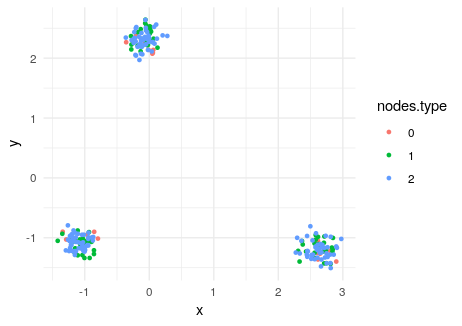
\includegraphics[scale=1]{sim_true.png}
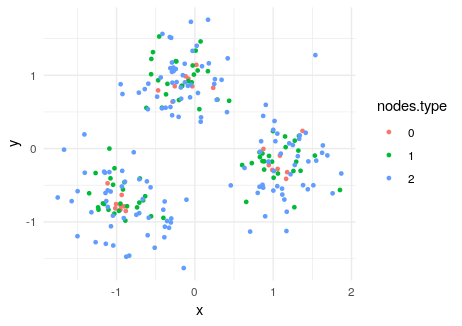
\includegraphics[scale=1]{sim_t1.png}

3. histogram of pairwise distance from the previous simulation:\\
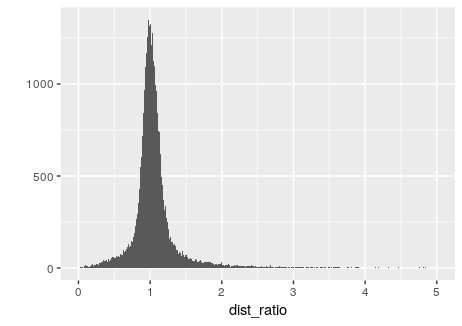
\includegraphics[scale=1]{hist_dist_ratio.png}
\end{document}